\documentclass{amsart}
\usepackage{amsmath}
\usepackage{amsthm}
\usepackage[foot]{amsaddr}
\usepackage{hyperref}
\usepackage{cleveref}
\usepackage[framed]{mcode}
\usepackage{mathrsfs}
\usepackage{mathalfa}
\usepackage{tikz}
\usepackage{units}
\usetikzlibrary{matrix}
\usetikzlibrary{shapes.geometric}
\usetikzlibrary{shapes.misc}
\usetikzlibrary{decorations.pathmorphing}
\usetikzlibrary{arrows}
\usetikzlibrary{backgrounds}
\usetikzlibrary{positioning}
\usetikzlibrary{fadings}
\DeclareMathOperator*{\argmin}{arg\,min}
\DeclareMathOperator*{\supp}{supp}
\DeclareMathOperator*{\acos}{acos}

%\title{An Application of Regularization for Radially Symmetric Linear Inverse Problems}
\title{Estimating and Quantifying Uncertainty for the Reconstruction of a Point Spread Function from the Image of an Edge}
\author{Kevin T. Joyce$^*$} \label{A1}
\author{Aaron Luttman$^\dagger$} \label{A2}
\author{Johnathan M. Bardsley$^*$}  \label{A3}
\address[$^*$]{Department of Mathematics, University of Montana, Missoula, MT 59812-0863 USA}
\address[$^\dagger$]{Mathematics \& Data Analysis, National Security Technologies, LLC, P.O. Box 98521, M/S NLV078, Las Vegas, NV 89193-8521 USA}

\theoremstyle{plain}
\newtheorem{thm}{Theorem}[section]
\newtheorem{lem}[thm]{Lemma}
\newtheorem{prop}[thm]{Proposition}
\newtheorem{cor}[thm]{Corollary}
\newtheorem{defn}[thm]{Definition}

\begin{document} 
\renewcommand{\bar}{\overline}
\renewcommand{\hat}{\widehat}
\renewcommand{\tilde}{\widetilde}
\newcommand{\eps}{\varepsilon}
\newcommand{\del}{\partial}
\newcommand{\RR}{\ensuremath{\mathbb R}}
\newcommand{\vect}[1]{\boldsymbol{#1}}
\newcommand{\DD}{\ensuremath{\mathfrak D}}
\newcommand{\K}{\ensuremath{\mathscr K}}
\newcommand{\R}{\ensuremath{\mathscr R}}
\newcommand{\HH}{\ensuremath{\mathscr H}}

\nocite{bachman1966,rudin1991,tikhonov1963,hansen1994,morozov1993,bracewell,abramowitz1972,morton2005numerical} % Show all references

\begin{abstract}
%  A model for translation invariant image blur is integral convolution with a point spread function (PSF) specific to the imaging instrument and the physics of the scene.
%  Standard techniques for estimating the PSF involve imaging a bright point source; however, in certain applications such as high energy X-ray radiography, imaging a bright point source is not feasible.  
%  However, when the PSF has radial symmetry, the estimation is possible from an image of an aligned edge, but the problem is ill-posed.
%  This work develops a framework for regularizing the estimation of a radially symmetric PSF.
  This work develops a framework for estimating the PSF of an imaging system where an impulse response is not available (e.g. X-Ray radiography).
  The method requires the assumption that the PSF exhibits radial symmetry.
  We derive a stochastic model that assumes that the PSF is an autocorrelated Gauss-Markov random field, then perform a change of variables and solve the inverse problem on the radial representation of the PSF for estimation.
  We carry out this numerically for a synthetic example as well as for actual radiographic data from the U.S.~Department of Energy's dual-beam X-ray radiographic diagnostic system Cygnus
  located at the Nevada National Security Site (NNSS) research complex.
\end{abstract}

\maketitle

%%%%%%%%%%%%%%%%%%%%%%%%%%%%%%%%%%%%%%%%%%%%%%%%%%%%%%%%%%%%%%%%%%%%%%%%%%%%%%%%
%                                                                              % 
%                                introduction                                  % 
%                                                                              % 
%%%%%%%%%%%%%%%%%%%%%%%%%%%%%%%%%%%%%%%%%%%%%%%%%%%%%%%%%%%%%%%%%%%%%%%%%%%%%%%%
\section{Introduction} \label{introduction}
test

\section{Model Formulation}
Consider a model for imaging an opaque object whose profile is indicated by $E \subseteq \RR^2$, which is subject to blurring by convolution with a PSF $k:\RR^2 \to \RR^2$. 
The blurry image $f$ is given by
\begin{equation}
  f(x,y) = \int_{-\infty}^\infty\int_{-\infty}^\infty k(x-s,y-t)\chi_E(s,t)dsdt,
  \label{blur_model}
\end{equation}
where $\chi_E$ is the indicator function $\chi_E(s,t) = 1$ for $(s,t) \in E$ and 0 otherwise. 
If we assume that $E$ represents a sharp edge with a known location fixed at $x=0$, then $\chi_E(s,t)$ depends only on $s$ and is given by $\chi_E(s) = 1$ if $x\ge0$ and $0$ if $x <0$. 
Using the symmetry of convolution, it follows that the response depends only on horizontal position, $x$, and \eqref{blur_model} reduces to 
\begin{equation}
  f(x) 
  = \int_{-\infty}^\infty\int_{-\infty}^\infty k(s,t)\chi_E(x-s)dsdt \label{blur_model2}.
\end{equation}

%\begin{figure}[h]
%\begin{center}
%\includegraphics[width=.65\textwidth]{figures/2d_radial_convolution.pdf}
%\caption{A circularly symmetric kernel superimposed over an opaque profile of an ideal sharp edge. }
%\end{center}
%\end{figure}

As an operator equation,
\begin{equation}
  f = \mathcal A k \label{operator1}
\end{equation}
where $f(x)$ is a \emph{line-out} of the blurred edge and $\mathcal A$ is the integral blurring operator of the kernel $k(s,t)$.

\section{Radial blurring as a Fredholm integral operator of the first kind}
For this work, we assume  $k$ is or radially symmetric. 
(I need a reference here for why this is reasonable).
Hence, one can reduce the dimension of the solution by a change of variables, $T:\RR^2 \to \RR^2$ so that $T(r,v) = (s,t)$ is invariant with respect to $r(s,t) = (s^2 + t^2)^{1/2}$.
Equation \eqref{blur_model2} is thus written
\begin{equation}
  f(x) = \iint_{U(r,v)} \rho(r) \chi_E\big(x - s(r,v)\big) \big|dT\big|. 
  \label{gen_problem}
\end{equation}
We remark that so long as symmetry can be expressed as invariance with respect to precomposition with the some map $r:\RR\to U$, \eqref{gen_problem} represents a reduction of dimension in the estimation.
As will be seen sampling section, this reduction allows for a marginalization technique that includes computations which in two dimensions would be unfeasible.
If we take $T$ to be the standard polar coordinates map, $s=r\cos v, t=r\sin v$, then \eqref{gen_problem} becomes
\begin{equation}
  f(x) = \int_0^\infty\rho(r) \left( \int_{-\pi}^{\pi} \chi_E(x - r\cos v)d v \right)rdr.
  \label{acos_form}
\end{equation}
Put $g(x,r)=\int_{-\pi}^{\pi} \chi_E(x - r\cos v)d v$, and note that we have reduced \eqref{blur_model2} to solving an integral equation with kernel $k(x,r) = g(x,r) r$.  
We will show that this kernel is continuous, hence \eqref{fredholm_problem} is an Fredholm integral equation of the first kind,
\begin{equation}
  f(x) = \int_0^\infty\rho(r) g(x,r) r dr. \label{fredholm_problem}
\end{equation} 
As an inverse problem, Fredholm integral equations of the first kind are known to be ill-posed.

To see the continuity of $g(x,r)$, note that for fixed $x$ and $r$, $g(x,r)$ is the measure of the set in $v\in \RR$ so that $x \ge r \cos v$.  
There are three cases to consider depending on $x$: $x \le -r$, $|x| < r$, and $x > r$. 
See \Cref{g_cases}.
The resulting analytic representation of $g$ is
\begin{equation}
  g(x,r) = \begin{cases}
    0 &\text{ if } x < -r\\
    2(\pi - \acos(x/r)) &\text{ if } |x| < r\\
    2\pi & \text{ if } x>r
  \end{cases},
  \label{g_form}
\end{equation}
which is indeed continuous.  Note that for each fixed $x$, however, $g$ is not differentiable in $r$ at $r=x$.  
This means that for numerical integrals involving $g$, bounds based on Taylor series can only guarantee convergence on the order of the discretization grid.  
See \Cref{g_figure} for plots of $g(x,r)$.
\begin{figure}[h]
\begin{center}
%\begin{tikzpicture}[scale=.8]
%  \draw (-.2,0) -- ({2*pi+.2},0) node[right]{\footnotesize$v$};
%  \draw (0,-2.5) -- (0,2.5) node[above]{\footnotesize$r\cos v$};
%
%  \draw[dotted] (0,-2.25) node[left] {\footnotesize$x<-r$}-- ({2*pi+.2},-2.25);
%  \draw[dotted] (0,-1) node[left] {\footnotesize$|x|\le r$}-- ({2*pi+.2},-1);
%  \draw[dotted] (0,2.25) node[left] {\footnotesize$x>r$}-- ({2*pi+.2},2.25);
%  \draw[very thick,red] (0,2.25) -- ({2*pi+.2},2.25);
%
%  \draw[domain=0:{2*pi}] plot (\x,{2*cos(180/pi*\x)});
%  \draw[very thick,red] ({4*pi/6},-1) -- ({8*pi/6},-1);
%\end{tikzpicture}
%\hspace{2cm}
\begin{tikzpicture}[scale=.8]
  \draw (0,-2.2) -- (0,2.2);
  \draw (-3,0) -- (3,0);
  \draw[dotted] (-2.5,-2.2) node[below]{\footnotesize$x<-r$} -- (-2.5,2.2);
  \draw[dotted] (2.5,-2.2) node[below]{\footnotesize$x>r$} -- (2.5,2.2);
  \draw[dotted] (-1,-2.2) node[below right]{\footnotesize$|x|\le r$} -- (-1,2.2);

  \draw (0,0) circle[radius=2];
  \draw[very thick,red,domain=120:240] plot ({2*cos(\x)},{2*sin(\x)});
  \draw (0,0) -- (-1,{sqrt(3)});
  \draw (.3,0) node[above right]{$v$} arc [radius=.3,start angle=0,end angle=120];
\end{tikzpicture}
\caption{ $g(x,r)$ represented as the arc measure of $v$ in $[-\pi,\pi]$ where $x > r\cos v$. }\label{g_cases}
\end{center}
\end{figure}


\begin{figure}[h]
  \begin{center}
  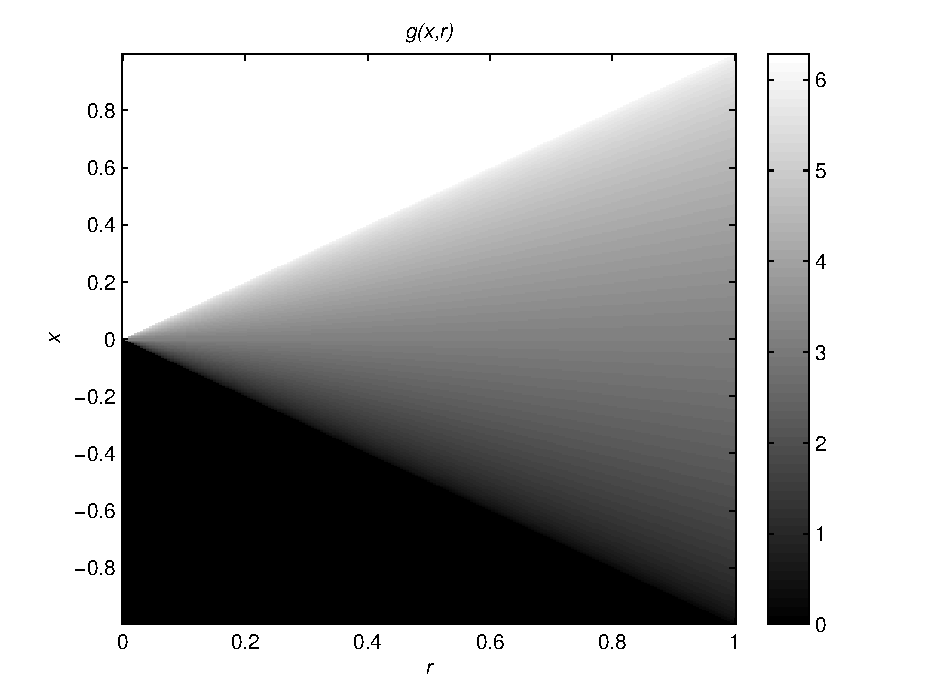
\includegraphics[width=.5\textwidth]{figures/g_function.pdf}
  \includegraphics[width=.45\textwidth]{figures/line_outs.pdf}
  \caption{Graphical representations of $g(x,r)$. } \label{g_figure}
  \end{center}
\end{figure} 

\section{Stochastic Model for Prior Assumptions and Measurement Error}
Since data is typically collected on a finite regular grid, we model the discrete realization of the line-out on $n$ regularly spaced points $x_i\in [-1,1]$ and $f(x_i)$.  
We require that $n$ be odd and that the central point corresponds to the point of symmetry of the line-out (i.e. the location of the edge).  
We also assume that measurement of the true signal is subject to error that we model with identical and independent Gaussian random variables $\epsilon_i$ with $ E \epsilon_i = 0$ and $E \epsilon_i^2 = \lambda^{-1}$.  
Using \eqref{fredholm_problem}, the forward data-measurement model is
\begin{equation}
  f(x_i) = \int_0^\infty \rho(r)g(x_i,r)\,rdr +  \epsilon_i. \label{stochastic_inv_problem} 
\end{equation}

Following the Bayesian approach outlined in \cite{stuart2010}, we assume a priori that $\rho$ is random element in a separable Hilbert space with $E \rho = 0$ and $\mathrm{Cov} \rho = \delta^{-1}Q$.
Using Bayes formula, we form a posterior density to estimate  and quantify the uncertainty.
If we further assume that $\rho$ is Gaussian, it has a density of the form
\begin{equation}
  \pi_0(\rho) \propto \exp\left(-\frac {\delta}2 \left\|Q^{-1/2} \rho\right\|^2_H \right). 
  \label{prior_density}
\end{equation}
Bayes' formula gives the posterior density
\begin{equation}
  \pi_f(\rho) = \propto \lambda^{n/2} \delta^{\dim H /2}\exp\left( -\frac {\lambda}2 \left\| \vect f - \mathcal G \rho \right\|^2_{R^n} - \frac \delta2 \| Q^{-1/2} \rho \|^2_{H} \right),
  \label{posterior_density}
\end{equation}
where $\vect f$ is the $n\times 1$ vector of measured line-out points, $\mathcal G : H \to \RR^n$ is the Fredholm integral operator restricted to the measurement grid.
Note that a maximum a posteriori (MAP) estimator of \eqref{posterior_density} is readily obtained by minimizing the negative argument of the exponential, which is quadratic and has a unique minimum
\begin{equation}
  \hat \rho_{MAP} = \left( \lambda \mathcal G^* \mathcal G + \delta Q^{-1}\right)^{-1} \mathcal G^* \vect f.
  \label{map_estimate}
\end{equation}

Prior beliefs about $\rho$ are modeled through the correlation structure $Q$. In particular, we implicitly assume that the prior distribution of $\rho$ is such that 
\begin{equation}
  \begin{cases}
    \displaystyle{\delta \left( \frac{\partial}{\partial r} \left(\kappa(r)r \frac{\partial}{\partial r}\right)\right)^2 \rho(r) \sim \mathcal N (0,\delta I),}\\
    \displaystyle{\rho(0) < \infty,\,\,\rho'(0) = 0,\,\,\lim_{r\to\infty}r\rho(r)\rho'(r) = 0.}
  \end{cases}
  \label{biharmonic_prior}
\end{equation}

\section{Sampling with Marginalization}

%\section{Numerical Simulation on an Analytic Example}
%A radially symmetric two dimensional Gaussian PSF has the form
%\begin{equation}
%  \rho(r) = (2\pi\sigma^2)^{-1} e^{\frac{-r^2}{2\sigma^2}} 
%  \label{radial_gaussian}
%\end{equation}
%and it can be analytically shown (See Appendix.)  that the blurring operator with this kernel results in an error function
%\begin{equation}
%  [\mathcal B \rho] (x) = \frac 1{\sqrt{2\pi}\sigma} \int_{-\infty}^x e^{-\frac{s^2}{2\sigma^2}}\,ds.
%  \label{analytic_edge}
%\end{equation}
%We simulate measured line-out edge data on a regular grid of $n$ points $x_i\in [-1,1]$ using \eqref{analytic_edge} and at each point adding computer realizations of independent zero mean Gaussian random variable. The simulated measurement error has variance such that the signal to noise ratio (SNR) is on the order of 30 - 50, i.e.
%\begin{equation}
%  \sigma_{noise} = \frac{ \| \mathcal B\rho \|}{\sqrt{n\cdot\mathrm{SNR}}}.
%  \label{noise_sigma}
%\end{equation}
%
%To calculate the MAP estimate of \eqref{posterior_density}, we discretize the integral operator \eqref{stochastic_inv_problem} using midpoint quadrature with $m$ points $r_j\in[0,1]$. 
%We assume that the scale of measured data compared to that of the kernel is such each improper integral is approximated on compact intervals and are rescaled to $x_i \in [-1,1]$ and $r_j \in [0,1]$.  
%To numerically estimate $\mathcal B$, we use midpoint quadrature and take $r_j$ to be the midpoints of $x_i$ in $[0,1]$,
%\begin{equation}
%  [\mathcal B \rho](x_i) \approx \frac{1}{m}\sum_{k=1}^m \rho(r_j) g(x_i,r_j) r_j h. 
%  \label{fredholm_discretization}
%\end{equation}
%Note that there are $m = (n-1)/2$ points $r_j$. 
%So, if we denote the $n\times m$ discretization matrix as $B$, this ensures that the symmetry $g(x_i,r_j)$ does not lead to potential collinearity in columns of $B$. 
%See \figref{g_figure}.
%
%The differential operator in the prior is discretized using finite central differences for the \emph{non-squared} radial Laplacian similar to the treatment in \cite{morton2005numerical}.
%Denote the discretization matrix as $P$ with row-vectors $\vect P_j$.  
%Then, for $j>1$ if $a_{j\pm1/2} = \kappa(r_j \pm h/2)(r_j \pm h/2)$ and $\rho_j = \rho(r_j)$, one obtains
%\begin{equation}
%  \vect P_j = \frac{1}{h^2} \Big[ a_{j+1/2}(\rho_{j+1} - \rho_j) - a_{j-1/2}(\rho_{j} - \rho_{j-1})\Big]
%  \label{laplacian_discretization}
%\end{equation}
%or as a matrix stencil
%\begin{equation}
%  \frac{1}{h^2}
%  \begin{bmatrix}
%    -(a_{j-3/2} + a_{j-1/2}) & a_{j-1/2} & 0             \\
%    a_{j-1/2} & -(a_{j-1/2} + a_{j+1/2}) & a_{j+1/2}     \\
%    0 & a_{j+1/2} & -(a_{j+1/2} + a_{j+3/2}) \\
%  \end{bmatrix}
%  \begin{bmatrix}
%    \rho_{j-1} \\
%    \rho_{j}   \\
%    \rho_{j+1} \\
%  \end{bmatrix}.
%  \label{laplacian_discretization_stencil}
%\end{equation}
%The left boundary has a zero derivative condition, so when $j = 1$
%\begin{equation}
%  P_j = \frac{2}{h^2} \Big[ a_{j+1/2}(\rho_{j+1}-\rho_j) \Big].
%  \label{prior_left_boundary}
%\end{equation}
%The right zero boundary condition is satisfied by setting $\rho_{n+1} = 0$ and omitting the bottom row.
%
%The final discretized prior is given by $L := P^2$.  
%Given $\lambda$ and $\delta$, we are now in a position to construct a discrete MAP estimate 
%\begin{equation}
%  \vect{\hat \rho}_{MAP} = \argmin_{\vect \rho\in\RR^m} \left(\frac \lambda 2 \|\vect f - B \vect \rho\|^2 + \frac \delta2 \|\delta L \vect \rho\|^2\right)
%  \label{discrete_objective}
%\end{equation}
%which, as a quadratic form, has a unique solution (up to the ratio $\frac \delta\lambda$) that satisfies
%\begin{equation}
%  \left(B^TB + \frac{\delta}{\lambda} L\right)\hat\rho = B^T f.
%  \label{normal_equation}
%\end{equation}
%Since we know the analytic output of blurring, we can select the optimal ratio $\frac{\delta}{\lambda}$ that minimizes the absolute relative error to the true solution.  
%We remark that the factor of $\frac 1{h^2}$ in $L$ can be omitted when forming $L$ by absorbing it into the term $\alpha = \frac\delta\lambda$.
%
%The simulation was carried out in \texttt{MATLAB} with three anisotropy functions
%\begin{align} 
%  k_1(r) &\equiv 1 \\
%  k_{norm}(r) &= \frac{b-1}{1-\Phi(-ba)}(\Phi(b(r-a))-\Phi(-ba))\\
%  k_{cos}(r) &= 
%  \begin{cases}
%    \frac{b-1}2(\cos(\pi(r/a-1))+1)+1 & r<a\\
%    b & r\ge a.
%  \end{cases}
%\end{align}
%The first function introduces no anisotropy.
%The second function is a shifted and scaled cumulative distribution function for a standard Gaussian so that $k_{norm}(0) = 1$, its point of symmetry occurs at $r=a$, and $k_{norm}(\infty) = b$.
%The third function is similar to the second, only the transition is given by a trigonometric function. 
%See \figref{anisotropy_functions}.
%\begin{figure}[h]
%  \begin{center}
%    \includegraphics[width=\textwidth]{figures/anisotopy_functions.pdf}
%    \caption{Two prior anisotropy functions with $a=.35$ and $b=10$. } \label{anisotropy_functions}
%  \end{center}
%\end{figure} 
%\begin{figure}[h]
%  \makebox[\textwidth][c]{\includegraphics[width=1.7\textwidth]{figures/500_reconstructions_with_anisotropy.pdf}}
%    \caption{Three MAP reconstructions with square radial Laplacian and two anisotropy functions. The known analytic PSF is the thin blue line and the gray region is the central 90\% of reconstructions at each $r$.} \label{map_reconstructions}
%\end{figure} 
%
%In \figref{map_reconstructions}, note that the peak of the reconstruction is consistently over estimated.  
%We suspect that this is due to edge effects, although at this time do not have rigorous justification for this.  
%In the next section, we present a technique that that transforms the data in such a way the peak of the PSF is reconstructed away from the boundary.
%This introduces bias in our estimate, but empirically corrects the apparent edge effect on this example.
%
%\section{Biased Edge Correction Transformation}
%(This section is also a template and does not give much rigorous motivation for why this works.)
%In the discrete form introduced in the last section, reconstructions of the PSF near $r = 0$ significantly overestimated the known analytic solution. 
%If accurately estimating the peak of the PSF is important, and we assume that the peak occurs at $r=0$ and that the overestimation in the last section is indeed a boundary artifact, then we can proceed by trying to mitigate boundary effects.
%We employ a technique similar to one used image reconstruction that reconstructs the PSF so that its peak is away from the boundary.
%
%In particular, for a fixed $\beta>0$, we transform the line-out data by a non-linear operator
%\begin{equation}
%  [H_\beta f](x) = \begin{cases}
%    f(x+\beta) & x\le 0\\
%    f(x-\beta) + (f(\beta) - f(-\beta)) & x>0.
%  \end{cases}
%\end{equation}
%%Due to the assumed symmetry of the PSF, the noise free line-out has point-symmetry about the point $f(0)$. 
%Note that the function $[H_\beta f](x)$ is continuous provided $f$ is continuous.
%See \figref{edge_transformation} for a schematic of the transformation on a noise free line-out.
%\begin{figure}[h]
%  \begin{center}
%    \makebox[\textwidth][c]{\includegraphics[width=1.1\textwidth]{figures/edge_correction_schematic.pdf}}
%    \caption{A schematic of the action of the edge correction transformation $H_\beta$ on a noise free line-out $f$. PSF reconstruction on $[H_\beta f](x)$ results in a PSF whose peak is to the right of $r=0$.} \label{edge_transformation}
%  \end{center}
%\end{figure} 
%
%We now solve the biased inverse problem
%\begin{equation}
%  [H_\beta f](x_i) = \int_0^\infty \rho(r)g(x_i,r)\,rdr +  \epsilon_i. \label{biased_inv_problem} 
%\end{equation}
%The resulting reconstruction will have a peak to the right of $r=0$. 
%We then truncate the solution to the left of the peak, and rescale the estimate so that its numeric integral is one.
%For this to make any sense, we need to show how the solution to this relates to the solution to the original problem \eqref{stochastic_inv_problem}, and ideally that the solutions coincide as $\beta \to 0$. 
%This theory is yet to be worked out.
%
%This has been implemented in \texttt{MATLAB} on the synthetic example in the last section and the results are presented in \figref{edge_corrected_reconstruction}.
%\begin{figure}[h]
%  \begin{center}
%  \makebox[\textwidth][c]{\includegraphics[width=1.7\textwidth]{figures/500_reconstructions_with_edge_correction.pdf}}
%    \caption{Three MAP reconstructions with square radial Laplacian and two anisotropy functions with the edge correction operator applied to the line out data with $\delta = 2h$. The known analytic PSF is the thin blue line and the gray region is the central 90\% of reconstructions at each $r$.} \label{edge_corrected_reconstruction}
%  \end{center}
%\end{figure} 

%\newpage
%\appendix
%\section{Abel Transform Formulation}
%Alternative approaches reduce \eqref{inv_problem} by expressing the action of $A$ as iterated integration.  
%I.e.,
%\begin{equation}
%  f(x) 
%  = \int_{-\infty}^\infty\chi_E(x-s)\int_{-\infty}^\infty k(s,t)dtds
%  =: \int_{-\infty}^x\ell(s)ds, \label{inv_problem}
%\end{equation}
%where $\ell(s)$ is the marginal distribution of the blurring kernel in $s$.
%To see the action of $A$ on $\rho$, we express the integral in $\ell$ in terms of $r$, by the change of variables $r=(s^2 + t^2)^{-1/2}$, 
%\begin{align}
%  \ell(s) 
%  &= \int_{-\infty}^\infty k(s,t)dt \nonumber\\
%  &= 2\int_{0}^\infty \rho(\sqrt{s^2 + t^2})dt \nonumber \\ 
%  &= 2\int_{|s|}^\infty \rho(r)\frac{r}{\sqrt{r^2 - s^2}} dr. \label{abel_transform}
%\end{align}
%
%We note that the inner integral is the Abel transform of $\rho$, which is commonly encountered in imaging problems where radial geometry interacts with non-radial geometry.  
%See the references in \cite{knill93}.  
%This leads to the following explicit representation of the operator equation \eqref{operator1}
%\begin{equation}
%   f(x) = \int_{-\infty}^x\int_{|s|}^\infty \rho(r) \frac{r}{(s^2 - t^2)^{1/2}}\,drdt.
%   \label{abel_form}
%\end{equation}
%Note that this formulation is problematic for standard numerical discretization techniques due to singularities in the integrand of the Abel transform. 
%We present a numerical integration scheme where the integrand of the Abel transform is evaluated on midpoints to avoid evaluation at the singularity.  
%
%Since data are usually only given on a closed rectangular region, we assume that the region is square and rescaled so $(x,y) \in [-1,1]\times[-1,1]$, and we assume that the scale of the image and kernel are such that integrating over this region is sufficient for approximating the infinite region. 
%We re-derive the integral equation on this domain to highlight what errors this assumption introduces into the discretization.
%That is,
%\begin{align}
%  f(x) 
%  &= \iint_{-\infty}^{\infty} \chi_{E}(x - s) k(s,y) dyds \nonumber \\
%  &= \int_{-1}^1\int_{-1}^{1} \chi_{E}(x - s) k(s,y) dyds + \eps\nonumber \\
%  &= \int_{-1}^{x} \int_{-1}^{1} k(s,y) dyds + \eps.
%\end{align} 
%
%We perform a variable substitution similar to \eqref{abel_transform}, however, note that the upper bound of integration depends on $s$.  We make another scale assumption so that integral is approximated by integrating only up to one.
%Hence,
%\begin{align}
%f(x)
%  &= 2\int_{-1}^{x} \int_{|s|}^{\sqrt{s^2+1}} \frac{\rho(r)r}{\sqrt{r^2 - s^2}} drds + \eps\nonumber \\
%  &= 2\int_{-1}^{x} \int_{|s|}^{1} \frac{\rho(r)r}{\sqrt{r^2 - s^2}} drds + \eps'\nonumber\\
%  &= 2\int_{-1}^{x} \ell(s) ds + \eps', \label{discrete_abel}
%\end{align} 
%where it is understood that $\ell$ in \eqref{discrete_abel} is the finite interval approximation of the one in \eqref{inv_problem}.
%
%We first consider evaluation of the Abel transform integral $\ell(s)$.  
%Note that $\ell(-s) = \ell(s)$ and is defined for $-1\le s \le1$. 
%Hence, a regular grid that uses this symmetry will have an even number of points if $0$ is in the grid or an odd number of points otherwise.  
%We consider the odd case.  
%Let $s_i = \frac in$ where $i=-n,-n+1,\dots,n$. 
%Note that $\ell$ is even, so if $j(i) = |i|$ then $j = 0,1,\dots,n$ and $\ell(s_{-i}) = \ell(-s_i) = \ell(s_i) = \ell(s_{j(-i)})$. 
%Hence, we evaluate $\ell$ only on $j$, and apply symmetry to define $s_{-i}$.
%We now apply the midpoint quadrature rule 
%\begin{equation}
%  \int_{s_{j}}^{s_{j+1}} \frac{\rho(r) r}{(r^2 - s^2)^{1/2}} 
%  = \frac 1n \frac{\rho(r_j) r_j}{(r_j^2 - s_j^2)^{1/2}} + E_j
%  \quad \text{ where }r_j = \frac{s_j + s_{j+1}}{2}.  \label{quad_rule}
%\end{equation}
%Hence, we evaluate $\ell(s_{j'})$ for $j' = 0,1,\dots,n$ by 
%\begin{equation}
%  \ell(s_{j'}) = \sum_{j=j'}^{n} \rho(r_j) \frac{r_j}{(r_j^2 - s_{j'}^2)^{1/2}}\frac 1n. \label{abel_discretization}
%\end{equation}
%
%This can be written as a matrix vector equation
%\begin{equation}
%  \vect \ell = h \vect K \vect \rho \label{mat_vec}
%\end{equation}
%where $h = \frac 1n$; $\vect K$ is an upper triangular $(n+1)\times (n+1)$ matrix whose $(j,j')$ entry is given by $r_j(r^2_j - s_{j'}^2)^{-1/2}$ when $j > j'$ and $0$ otherwise; and the vector $\vect \rho$ has entries $\rho(r_j)$.
%A partial analysis of the errors in this estimate can be found in the Analysis of Abel Error section.
%
%\section{Abel Discretization Error Analysis}
%If we assume that the radially expressed kernel $\rho$ is twice differentiable, then the error term for the quadrature rule \eqref{quad_rule} has the bound
%$$
%  |E_j| \le \frac 1{24n^3} \left|\rho''(t_j)\phi_{j'}(t_j) + 2\rho'(t_j)\phi_{j'}'(t_j) + \rho(t_j)\phi_{j'}''(t_j)\right|
%$$
%where $\phi_{j'}(r) = r(r^2 - s_{j'}^2)^{-1/2}$, $\phi_j'(r) = -s_{j'}^{2}(r^2 - s_{j'}^2)^{-3/2}$ and $\phi_{j'}''(r) = 3 s_{j'}^2 r (r^2 - s_{j'}^2)^{-5/2}$, for some $s_j<t_j<s_{j+1}$.
%The absolute error in our estimate for $\ell(s_{j'})$ is given by
%$$
%  \left|\sum_{j=j'}^{n-1} E_j\right|. %\le \sum_{j=j'}^{n-1} \frac 1{24n^3} \left(\rho''(t_j)\phi_i(t_j) + 2\rho'(t_j)\phi_i'(t_j) + \rho(t_j)\phi_i''(t_j)\right)
%$$
%
%If we assume that $M$ is an upper bound for each derivative of $\rho$, and denote $h = \frac 1{n}$ and $d_j = (t_j^2 - s_{j'}^2)^{1/2}$, then an upper bound for the error is given by 
%\begin{align}
%  \sum_{j=j'}^{n-1} |E_j| 
%  &\le M \sum_{j=j'}^{n-1} \frac {h^3}{24} \Big(\frac{t_j}{d_j} - \frac{2s_{j'}^{2}}{d_j^3} + \frac{3 s_{j'}^2 t_j}{ d_j^5 } \Big). \label{error_bound}
%\end{align} 
%
%%\hrule
%%The following are notes in trying to analyze \eqref{error_bound}.
%%
%%When $j'$ is near $n$, then $s_{j'} \approx O(1)$ and $t_j\approx O(1)$, so $d_j \approx O(h)$ and we are summing over $O(1)$ terms so 
%%$$
%%  \sum_{j=j'}^{n-1} |E_j| \approx O(|E_j|) \le O(h^{-2}).
%%$$ 
%%This is not a useful upperbound, but upon finding how sharp it is, we can say something.
%%
%%However, when $j'$ is near $0$, we must consider terms ranging from $j'$ to $n-1$.  For the terms where $j$ is near $j'$, then $|t_j - s_{j'}| \approx O(h)$ implies $d_j \approx O(h)$, and thus $|E_j| \approx O\left(s_{j'}^3h^{-2}\right)$
%%Moreover then $s_{j'} \approx O(h)$. If we assume that these terms dominate, and we are summing over $O(n)$ terms so
%%$$
%%  \sum_{j=j'}^{n-1} |E_j| \approx O(h^{-1}|E_j|) \le O(1).
%%$$
%
%\section{Comparison of Forward Numerical Approximations}
%
%An independent two dimensional Gaussian kernel is given by the product of one dimesional Gaussian densities 
%\begin{equation}
%  k(s,t) = \phi_\sigma(s) \, \phi_\sigma(t),
%\end{equation}
%where $\phi(s) = (2\pi\sigma^2)^{-1/2}e^{-(s/\sigma)^2}$. The forward blur of an edge is thus 
%\begin{align}
%  f(x) 
%  &= \int_{-\infty}^\infty \int_{-\infty}^\infty k(x,s) \chi_E(x-s)dsdt \nonumber\\
%  &= \int_{-\infty}^\infty \phi_\sigma(t) dt\cdot \int_{-\infty}^x \phi_\sigma(s) ds \nonumber\\
%  &= \Phi_\sigma(x)
%\end{align}
%where $\Phi_\sigma$ is the cumulative density function (CDF) for the Gaussian density.
%
%We numerically estimate the Abel integral using midpoint quadrature on each integral, i.e.
%\begin{equation}
%  f_{abel}(x_i) = \frac{1}{n^2} \sum_{j=1}^{i-n} \sum_{k=1}^n \frac{ \rho(r_{k_j}) r_{k_j}}{(r_{k_j}^2 - s_j^2)^{1/2}}
%\end{equation}
%and
%\begin{equation}
%  f_{Fred}(x_i) = \frac{1}{n}\sum_{k=1}^n \rho(r_j) g(x_i,r_j) r_j
%\end{equation}
%
%%See the Abel discretization document(\texttt{abel\_discretization.pdf}) for details. 
%%\begin{figure}[h]
%%\begin{center}
%%\begin{tikzpicture}[scale = .5]
%%  \draw (-10,0) -- (10,0);
%%  \node[above] (o) at (0,0) {0};  
%%  \foreach \x in {-9,-8,...,10} {
%%    \draw[shift={(\x,0)}] (0pt,-2pt) -- (0pt,2pt);
%%  };
%%  \node[above] (l) at (-10,0) {-1};
%%  \node[above] (r) at (10,0) {1};
%%  \draw[-latex] (-9,-1) node[below] {$x_i$} -- (-9,-2pt);
%%  
%%  \foreach \x in {0,1,...,10} {
%%    \draw[shift={(\x,0)}] (-2pt,-2pt) -- (2pt,2pt);
%%    \draw[shift={(\x,0)}] (-2pt,2pt) -- (2pt,-2pt);
%%  };
%%  \draw[-latex] (-1,-.75) node[below] {$s_j$} -- (0,-2pt);
%%
%%  \foreach \x in {.5,1.5,...,9.5} {
%%    \fill (\x,0) circle (2pt);
%%  };
%%  \draw[-latex] (.5,-.75) node[below] {$r_{k_j}$} -- (.5,-2pt);
%%\end{tikzpicture}
%%\end{center}
%%\caption{ A diagram of the discretized variables in the numerical Abel blur. } \label{discretization}
%%\end{figure}
%%
%%We discretize \eqref{acos_problem} using midpoint quadrature so that 
%%\begin{equation}
%%  f_{acos}(x_i) =  \frac 1n\sum_{j=1}^n \rho(r_j) g(x_i,r_j) r_j,\label{acos_discretization}
%%\end{equation}
%%where $x_i = i/n$, $i=-n,\dots,n-1$ and $r_j= j/n$, $j=0,\dots,n-1$. Using $n = 200$ and $\sigma = .02$, the resulting numerical estimates resulting in errors
%%\begin{align}
%%  \frac{\|f_{abel}(x_i) - \Phi_\sigma(x_i)\|_{max}}{\|\Phi_\sigma(x_i)\|_{max}} &\approx 0.1694 \\ 
%%  \frac{\|f_{acos}(x_i) - \Phi_\sigma(x_i)\|_{max}}{\|\Phi_\sigma(x_i)\|_{max}} &\approx 0.1048.
%%\end{align}
%%
%See \figref{comparison} for a graphical comparison of each forward blur.  Both
%methods produce errors that appear to be on the same order as the discretization grid, but with the Abel transform performing
%consistently more poorly. 
%These results are not surprising, as standard quadrature errors are generally given in terms of a second derivative of the
%integrand, and in both cases the numerical integration involves an integrand that has an unbounded second derivative.
%(In the case of the Abel transform it is the integrand itself that is unbounded, and in the case of the Fredholm formulation, the kernel function $g$ has a discontinuous derivative along $s=t$.)
%
%\begin{figure}[h!]
%  \begin{center}
%  \includegraphics[width=.8\textwidth]{forward_compare.pdf}
%  \caption{Comparisons of numerical blurring with Gaussian kernel.} \label{comparison}
%  \end{center}
%\end{figure} 
%
%
\bibliographystyle{alpha}
\bibliography{edge_spread_report}
\end{document} 

